\documentclass[10pt,a5paper,twoside]{article}
\usepackage[top=12mm,bottom=26mm,outer=28mm,inner=14mm,foot=14mm]{geometry}
\usepackage{calc}
\usepackage{scrextend}
\deffootnote[1.5em]{0em}{1em}{\thefootnotemark\quad}
\renewcommand{\footnoterule}{%
  \kern -2.4pt
  \hrule width \textwidth height 0.4pt
  \kern 2pt
}

\usepackage{microtype,ellipsis}
\usepackage[ngerman]{babel}
\usepackage[utf8]{inputenc}
\usepackage[T1]{fontenc}
\usepackage[T2A,T1]{autofe}

\usepackage{textcomp}

\usepackage{amsmath,amssymb,nicefrac,amscd}
\usepackage{graphicx,float}
\usepackage{pdfpages}

\usepackage{enumitem}
\setitemize[1]{noitemsep,nosep,leftmargin=0.99em,label={--}}

\usepackage{transparent}
\usepackage{csquotes}
\usepackage{siunitx}
\sisetup{per-mode=fraction,fraction-function=\nicefrac}
\DeclareSIUnit[number-unit-product=\,]\uhr{Uhr}
\DeclareSIUnit[number-unit-product=\,]\zoll{Zoll}

\usepackage{hyperref}

\usepackage{todonotes}

\newenvironment{problem}[1]{\paragraph*{#1}}{}

%\marginparwidth 40pt
%\textwidth=140mm
%\textheight=206mm


\title{Denkaufgaben für Kinder von 5 bis 15}
 
\author{V.\,I.~Arnold
\vspace*{2cm}\\ 
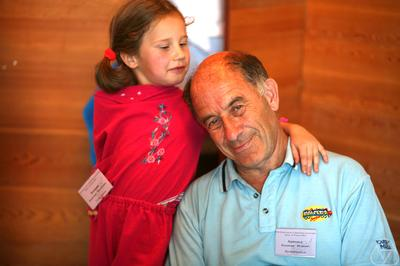
\includegraphics[width=12cm]{photo-arnold_small}
}

\date{}
\begin{document}
\includepdf[pages={2,3}]{"cover_de_DE"}

%\sloppy
\def\eps{\varepsilon}
%%\vskip7cm

%\maketitle
%\thispagestyle{empty}

%\newpage 
%\setcounter{page}{1} 
\begin{abstract}
\noindent Diese Sammlung enthält 77 Rätsel für die Förderung und Entwicklung einer Kultur des Denkens. Die Rätsel wurden von mir ausgewählt oder selbst erfunden. Die meisten erfordern keine besonderen Vorkenntnisse jenseits einer allgemeinen Schulbildung, aber manche von ihnen könnten auch einen Universitätsprofessor oder eine Uni\-ver\-si\-täts\-pro\-fes\-sorin herausfordern. 

Das Buch richtet sich an Schülerinnen und Schüler, Studentinnen und Studenten, Lehrerinnen und Lehrer und an Eltern. Mit anderen Worten, es richtet sich an all jene, die eine Kultur des Denkens als wesentlichen Teil der Persönlichkeitsentwicklung ansehen.
\end{abstract}
\clearpage

\section*{Vorwort}

Ich fing an diese Rätsel aufzuschreiben, nachdem mich im Frühling 2004 in Paris lebende Landsleute baten, ihre Kinder in der Förderung einer Kultur des Denkens zu unterstützen, so wie sie in Russland Tradition hat.

Ich bin fest davon überzeugt, dass diese Kultur des Denkens schon in der frühen Kindheit besonders durch selbstständiges Tüfteln unterstützt wird, über Fragestellungen, die einfach zu begreifen, aber nicht unbedingt einfach zu lösen sind. Solche Fragen findet man in dieser Sammlung, besonders empfehle ich die Aufgaben mit den Nummern 1, 3 und 13.

Meine lange Erfahrung hat mir gezeigt, dass oft die \enquote{schwächeren} Schü\-le\-rin\-nen und Schüler solche Fragen besser beantworten können als akademisch erfolgreichere Kinder. Denn für ihr Überleben auf der hinteren Schulbank handeln sie wie Figaro, der \enquote{mehr Kenntnisse und Berechnung gebrauchen mußte, bloß um zu bestehen, als man seit hundert Jahren gebraucht hat, um ganz Spanien zu regieren}.

Währenddessen verliert sich die gute Schülerin oder der gute Schüler zu oft in der Frage, was man denn jetzt zusammen multiplizieren muss. 

Ich habe auch feststellen können, dass ein fünfjähriges Kind solche Rätsel oft besser lösen kann als routine-verdorbene Schülerinnen und Schüler, diese wiederum besser als ambitiöse Universitätsstudierende (die schlechtesten Löser solcher Aufgaben sind auf jeden Fall Nobel- und Fields-Preisträgerinnen und -träger).

\clearpage
\section*{Anmerkungen zur deutschen Ausgabe}
Wir haben uns erlaubt, gewisse Denkaufgaben im hinteren Drittel des Buches mit zusätzlichen Hinweisen und einem neuen Bild zu versehen und im Vergleich zur englischen Übersetzung auch anders zu formulieren. Dies betrifft die folgenden Denkaufgaben:
52 (freier formuliert), 61 (Tipp eingefügt), 64 (freier formuliert) 74 (Bild und Erklärung ergänzt), 75-77 (Erklärungen ergänzt).

Des Weiteren haben wir am Ende des Buches ein kurzes Glossar mit Definitionen von im Buch verwendeten mathematischen Begriffen hinzugefügt.

Wir würden uns sehr freuen, Rückmeldungen zu den Denkaufgaben zu erhalten, um den Einsatz dieses Buches zu verbessern. Diese können von Lösungsvorschlägen zu den Aufgaben, der Erweiterung des Glossars, neuen Übersetzungen bis hin zu Ideen für eine andere Formulierung der Aufgaben und weiteren Erklärungen reichen. Rückmeldungen, Feedback, Kommentare und Verbesserungsvorschläge bitte an:
\href{mailto:info@imaginary.org}{\nolinkurl{info@imaginary.org}}.

\clearpage
\section*{Die Rätsel}

%\ 
%
%\vspace{0pt plus 12pt}
%\centerline{*\quad *\quad*}
%\vspace{.4\baselineskip}
%
%\

%
\begin{problem}{1.}
	Masha fehlen sieben Kopeken, um ein Lesebuch zu kaufen, Misha fehlt eine Kopeke. Auch wenn sie ihr Geld zusammenlegen, um das Buch gemeinsam zu kaufen, fehlt ihnen immer noch Geld. Wie viel kostet das Buch?
\end{problem}

\begin{problem}{2.}
	Eine Flasche mit Korken kostet 10 Kopeken. Die Flasche alleine kostet 9 Kopeken mehr als der Korken. Wie viel kostet die Flasche ohne Korken?
\end{problem}

\begin{problem}{3.}
	Ein Ziegel wiegt soviel wie ein Pfund und ein halber Ziegel. Was ist das Gewicht eines Ziegels?
\end{problem}

\begin{problem}{4.}
	Ein Löffel Wein wird von einem Fass in ein (nicht volles) Glas Tee gegossen und verrührt. Danach wird ein Löffel dieser jetzt gemischten Flüssigkeit aus dem Glas zurück in das Fass gefüllt. In beiden Behältern befindet sich also jeweils etwas einer fremden Flüssigkeit (im Glas ist auch Wein und im Fass auch Tee). In welchem Behälter ist das Volumen der fremden Flüssigkeit größer?
\end{problem}

\begin{problem}{5.}
	Zwei alte Damen gehen sich auf derselben Straße seit Sonnenaufgang entgegen. Die erste geht von $A$ nach $B$, die zweite von $B$ nach $A$. Sie treffen sich mittags, halten aber nicht an und gehen geradeaus mit derselben Geschwindigkeit weiter. Die erste Dame kommt in $B$ um \SI{16}{\uhr} an, die zweite erreicht $A$ um \SI{21}{\uhr}. Um wie viel Uhr war der Sonnenaufgang an diesem Tag?
\end{problem}

\begin{problem}{6.}
	Eine Frage in einem US-amerikanischen Standardtest lautet: Die Hypotenuse eines rechtwinkligen Dreiecks ist \SI{10}{\zoll} lang. Die Höhe des Dreiecks, gemessen von der Hypotenuse, beträgt \SI{6}{\zoll}. Berechne die Fläche des Dreiecks.

	Schüler in den USA hatten über ein Jahrzehnt lang mit dieser Aufgabe kein Problem. Als aber russische Studenten aus Moskau dieselbe Fragestellung angingen, war keiner von ihnen in der Lage, das Problem zu lösen - im Gegensatz zu ihren US-amerikanischen Kollegen, die korrekterweise \enquote{30\,Quadratzoll} als Antwort erhielten. Warum?
\end{problem}

\begin{problem}{7.}
	Wasja hat 2 Schwestern mehr, als er Brüder hat. Wie viel mehr Töchter als Söhne haben seine Eltern?
\end{problem}

\begin{problem}{8.}
	In der Mitte eines runden Teiches in Südamerika wächst jedes Jahr am 1.\,Juni eine Victoria-Regia-Blume. Ihr Stiel wächst vom Grund nach oben, die Blütenblätter liegen auf der Wasseroberfläche wie die einer Seerose. Die Oberfläche der Blume verdoppelt sich täglich, bis die Blütenblätter am 1.\,Juli die ganze Oberfläche des Teiches bedecken; danach fallen die Blütenblätter ab und die Samen sinken auf den Grund. An welchem Tag hat die Blume die Hälfte des Teiches bedeckt? 
\end{problem}

\begin{problem}{9.}
	Ein Landwirt muss einen Wolf, eine Ziege und einen Kohl über den Fluss bringen, aber das Boot ist so klein, dass er jedes Mal nur einen der drei mitnehmen kann. Der Wolf kann nicht mit der Ziege allein gelassen werden, die Ziege nicht mit dem Kohl. Wie kann er alle drei heil über den Fluss bringen? 
\end{problem}

\begin{problem}{10.}
	Eine Schnecke klettert während eines Tages \SI{3}{\cm} an einem Pfosten hoch. Bei Nacht jedoch schläft sie und rutscht jedes Mal \SI{2}{\cm} wieder herunter. Der Pfosten ist \SI{10}{\metre} hoch und ganz oben befindet sich ein leckeres Schnecken-Bonbon. In wie vielen Tagen wird die Schnecke das Bonbon erreichen?
\end{problem}

\begin{problem}{11.}
	Ein Landvermesser geht von seinem Zelt aus \SI{10}{\km} gen Süden und dann \SI{10}{\km} in Richtung Osten und trifft dort auf seinen Freund Bär. Von dort aus geht er \SI{10}{\km} gen Norden und erreicht wieder sein Zelt. Welche Farbe hat der Bär und wo spielt die Szene?
\end{problem}

\begin{problem}{12.}
	Ebbe war heute um \SI{12}{\uhr} mittags. Um wie viel Uhr wird morgen Ebbe am selben Ort sein?
\end{problem}

\begin{problem}{13.}
	Die ersten zwei Bände von Pushkins Werken stehen direkt nebeneinander auf einem Bücherregal. Die Seiten von jedem Band sind zusammen \SI{2}{\cm} dick und sowohl der vordere als auch der hintere Einband sind jeweils \SI{2}{\mm} dick. Ein Bücherwurm hat sich, rechtwinklig zu den Seiten, von der ersten Seite im ersten Band bis zur letzten Seite im zweiten Band durchgeknabbert. Wie lang ist die Spur des Bücherwurms? [Dieses topologische Problem mit seiner unerwarteten Antwort \SI{4}{\mm} ist unlösbar für viele Akademiker, aber manche Vorschüler lösen es ohne Probleme.]
\end{problem}

\begin{problem}{14.}
	Finde einen Körper mit der folgenden Draufsicht und Vorderansicht. Zeichne die Seitenansicht und deute unsichtbare Kanten durch gestrichelte Linien an. 
	\begin{figure}[H]
	\footnotesize
	\null\hfill
	\parbox{0.2\linewidth}{\centering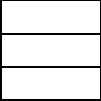
\includegraphics[scale=1]{taskbook-99}\\Draufsicht}
	\hfill
	\parbox{0.2\linewidth}{\centering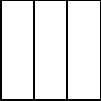
\includegraphics[scale=1]{taskbook-98}\\Vorderansicht}
	\hfill\null
	\end{figure}
\end{problem}

\begin{problem}{15.}
	Wie viele verschiedene Arten gibt es, die Zahl 64 in zehn ganze, positive Summanden zu zerlegen, wobei keiner grösser als 12 ist?
	%\newline
	[Antworten, die sich nur in der Reihenfolge der Zahlen unterscheiden, gelten als gleich.]
\end{problem}

\begin{problem}{16.}
	Wenn man gleichlange Stäbe (wie z.B.\ Dominosteine) übereinander legt, kann man einen Überhang der Länge $x$ erschaffen. Was ist die maximal er\-reich\-ba\-re Länge des Überhangs? 
	\begin{figure}[H]
	\centering
	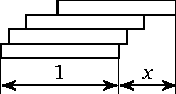
\includegraphics[scale=1]{taskbook-97}
	\end{figure}
\end{problem}

\begin{problem}{17.}
	Die Entfernung zwischen den Städten $A$ und $B$ beträgt \SI{40}{\km}. Zwei Fahrradfahrer verlassen gleich\-zei\-tig jeweils $A$ und $B$ und fahren sich direkt entgegen, einer mit \SI{10}{\km\per\hour} und der andere mit \SI{15}{\km\per\hour}. Eine Fliege fliegt mit einer Geschwindigkeit von \SI{100}{\km\per\hour} gemeinsam mit dem ersten Radfahrer von $A$ los, er\-reicht den zweiten Radfahrer, berührt seine Stirn und fliegt dann zurück zur Stirn des ersten Radfahrers, dann wieder zurück zum zweiten und so weiter, bis die beiden Köpfe der Radfahrer zusammenstoßen und die Fliege zwischen ihren Stirnen zerquetschen. 
	Wie viele Kilometer ist die Fliege insgesamt geflogen? 
	\begin{figure}[H]
	\centering
	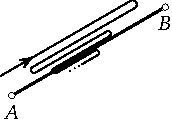
\includegraphics[scale=1]{taskbook-1}
	\end{figure}
\end{problem}

\begin{problem}{18.}
	Ein Dominostein verdeckt jeweils genau zwei Felder eines Schachbretts. Lege das gesamte Schachbrett bis auf zwei gegenüberliegende Eckfelder mit 31 weiteren Dominosteinen aus! [Ein Schachbrett besteht aus $8 \times 8 = 64$ quadratischen Feldern.]
	\begin{figure}[H]
	\centering
	\footnotesize
	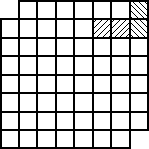
\includegraphics[scale=1]{taskbook-2}
	\end{figure}
\end{problem}

\begin{problem}{19.}
	Eine Raupe möchte in einem quaderförmigen Raum von einer Ecke (links unten am Boden) in die gegenüberliegende Ecke (oben rechts an der Decke) gelangen. 
	Finde den kürzestmöglichen Weg für die Raupe entlang der Wände. 
	\begin{figure}[H]
	\centering
	\footnotesize
	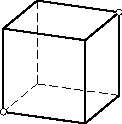
\includegraphics[scale=1]{taskbook-3}
	\end{figure}
\end{problem}

\begin{problem}{20.}
	Du hast zwei Behälter, einer fasst 5\,Liter, der andere 3\,Liter, und Wasser aus dem Wasserhahn. Wie kannst du in einem der Behälter genau einen Liter abmessen? 
	\begin{figure}[H]
	\centering
	\footnotesize
	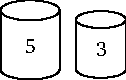
\includegraphics[scale=1]{taskbook-4}
	\end{figure}
\end{problem}

\begin{problem}{21.}
	In einer Familie gibt es fünf Köpfe und vierzehn Beine. Wie viele Menschen und wie viele Hunde sind in der Familie? 
\end{problem}

\begin{problem}{22.}
	Auf den Seiten $AB$, $BC$ und $CA$ des Dreiecks ABC werden nach außen hin gleichseitige Dreiecke konstruiert. Beweise, dass die Zentren ($*$) der so entstandenen Dreiecke ein gleichseitiges Dreieck bilden.
	\begin{figure}[H]
	\centering
	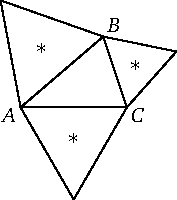
\includegraphics{taskbook-6}
	\end{figure}
\end{problem}

\begin{problem}{23.}
	Welche Vielecke können durch den Schnitt eines Würfels mit einer Ebene entstehen? Können wir ein Fünfeck, ein Siebeneck, ein regelmäßiges Sechseck erhalten? 
	\begin{figure}[H]
	\centering
	\footnotesize
	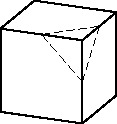
\includegraphics[scale=1]{taskbook-7}
	\end{figure}
\end{problem}

\begin{problem}{24.}
	Zeichne eine Gerade durch den Mittelpunkt eines Würfels, sodass die Summe der Quadrate der Entfernungen zwischen ihr und den acht Eckpunkten des Würfels (im Vergleich zu anderen Geraden durch die Mitte) möglichst a) groß b) klein ist.
\end{problem}

\begin{problem}{25.}
	Ein gerader kreisförmiger Kegel wird von einer Ebene so geschnitten, dass eine geschlossene Kurve entsteht. Zwei Kugeln sind dem Kegel so eingeschrieben, dass sie die Ebene berühren, eine in Punkt $A$ und die andere in Punkt $B$. Finde denjenigen Punkt $C$ auf der Schnittkurve des Kegels mit der Ebene, bei dem die Summe der Distanzen $CA + CB$ möglichst a) groß b) klein wird. 
	\begin{figure}[H]
	\centering
	\footnotesize
	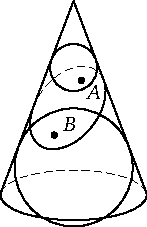
\includegraphics[scale=1]{taskbook-9}
	\end{figure} 
\end{problem}

\begin{problem}{26.}
	Die Erdoberfläche wird auf einen Zylinder projiziert. Der Mantel dieses Zylinders wird durch die Tangenten zu den Längengraden am Äquator geformt. Was ist grösser: die tatsächliche Fläche Frankreichs oder die projizierte Fläche?
	\begin{figure}[H]
	\centering
	\footnotesize
	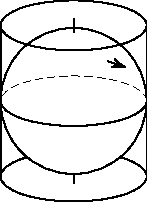
\includegraphics[scale=1]{taskbook-10}
	\end{figure}
\end{problem}

\begin{problem}{27.}
	Beweise, dass wenn $p$ eine ungerade Primzahl ist und die Zahl $2^{p-1}$ durch $p$ geteilt wird, der Rest 1 sein muss. (Beispiele: $2^2 = 3a +1,$ $2^4 = 5b+1,$ $2^6 = 7c+1, 2^{10} - 1 = 1023 = 11\cdot 93$). 
\end{problem}

\begin{problem}{28.}
	Eine \SI{10}{\cm} lange Nadel wird willkürlich auf eine linierte Seite Papier geworfen, dessen Linienabstand ebenfalls \SI{10}{\cm} beträgt. Dieser Vorgang wird $N$ (z.\,B.\ eine Million) mal wiederholt. 
	Kannst du eine Vorhersage treffen, wie oft die Nadel in etwa eine Linie kreuzen wird?
	\begin{figure}[H]
	\centering
	\footnotesize
	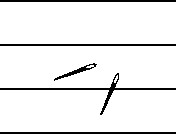
\includegraphics[scale=1]{taskbook-12}
	\end{figure}
	Es ist möglich, dieses Experiment mit nur $N=100$ auszuführen (wie ich es mit 10\,Jahren tat) anstatt einer Million. [Die Antwort auf diese Frage ist überraschend: $\frac2{\pi}N$. Selbst mit einer gekrümmten Nadel der Länge $a \cdot \SI{10}{\cm}$ ist die Antwort bei $N$ Würfen näherungsweise $\frac{2a}{\pi}N$. 
	Hierbei können wir die Zahl $\pi$ annähern durch $\pi \approx \frac{355}{113} \approx \frac{22}7.$]
\end{problem}

\begin{problem}{29.}
	Diejenigen Polyeder, bei denen alle Seitenflächen identisch sind, nennt man platonische Körper. Manche unter ihnen haben dreieckige Seitenflächen: Tetraeder (4 Seitenflächen), Oktaeder (8 Seitenflächen), Ikosaeder (20 Seitenflächen, 12 Ecken und 30 Kanten; dieses ist interessant zu zeichnen). 
	\begin{figure}[H]
	\centering
	\footnotesize
	\null\hfill
	\parbox{0.3\linewidth}{\centering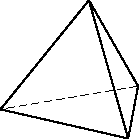
\includegraphics[scale=1]{taskbook-131}\\Tetraeder ($\text{tetra}= 4$)}
	\hfill
	\parbox{0.3\linewidth}{\centering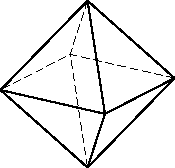
\includegraphics[scale=1]{taskbook-132}\\Oktaeder ($\text{octo}= 8$)}
	\hfill\null\\
	{\Huge ?}\\Ikosaeder
	\end{figure}
	%\newline\quad
	Überprüfe die folgende Behauptung: Die Anzahl der Seitenflächen eines konvexen Polyeders mit dreieckigen Seitenflächen ist gleich zwei mal der Anzahl der Ecken minus vier. 

	Noch ein platonischer Körper (es gibt insgesamt fünf):
	\begin{figure}[H]
	\centering
	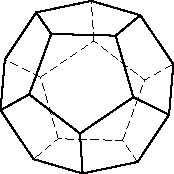
\includegraphics{taskbook-14}
	\end{figure}
\end{problem}

\begin{problem}{30.}
	Ein Dodekaeder ist ein konvexes Polyeder mit zwölf identischen, regelmäßigen fünfeckigen Seitenflächen. Es hat zwanzig Ecken und dreißig Kanten. (Im Übrigen befinden sich die Ecken des Dodekaeders jeweils in der Mitte der Seitenflächen eines Ikosaeders.)
	Finde fünf verschiedene Würfel im Inneren des Dodekaeders, sodass die folgenden Eigenschaften erfüllt sind: Die Ecken des Würfels sind auch Ecken des Dodekaeders, die Kanten des Würfels sollen Diagonalen der Seitenflächen des Dodekaeders sein. (Zur Erinnerung: Ein Würfel hat 12 Kanten, eine pro Seitenfläche des Dodekaeders.) 
	%Finde fünf verschiedene Würfel, die so in das Dodekaeder passen, dass ihre Ecken auch Ecken des Dodekaeders sind und ihre Kanten Diagonalen der Seitenflächen des Dodekaeders sind (ein Würfel hat 12 Kanten, eine pro Seitenfläche (?????)). 
	[Diese Frage wurde von Johannes Kepler gestellt, um Planetenbahnen zu beschreiben.]
\end{problem}

\begin{problem}{31.}
	Beschreibe das Schnittvolumen von zwei Tetraedern, die auf folgende Art in einem Würfel liegen: Die Ecken des Tetraeders sind auch Ecken des Würfels, die Kanten des Tetraeders sind Diagonalen der Seitenflächen des Würfels.
	%die in einen Würfel passen, sodass ihre Ecken auch Ecken des Würfels sind und ihre Kanten Diagonalen der Seitenflächen. 
	Welchen Bruchteil des Würfel-Volumens stellt dieser Schnitt dar?
\end{problem}

\begin{problem}{31\textsuperscript{bis}.} 
	Konstruiere den Schnitt eines Würfels und einer Ebene, die durch drei gegebene Punkte auf den Würfelkanten geht (siehe Zeichnung). [Zeichne das Vieleck, das die Schnittfläche bildet.]
	\begin{figure}[H]
	\centering
	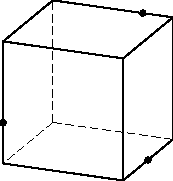
\includegraphics{taskbook-15}
	\end{figure}
\end{problem}

\begin{problem}{32.}
	Wie viele Symmetrien hat ein Tetraeder? Wie viele hat ein Würfel? Ein Oktaeder? Ein Ikosaeder? Ein Dodekaeder? Eine Symmetrie ist eine Umwandlung, die ein Objekt auf sich selbst abbildet, also insbesondere die Längen des Objektes erhält. 
	Wie viele davon sind Drehsymmetrien, wie viele Spiegelsymmetrien?
\end{problem}

\begin{problem}{33.}
	Wie viele verschiedene Arten gibt es, einen Würfel mit 6 verschiedenen Farben $(1,\dotsc, 6)$ [eine pro Seite] anzumalen? Würfel, die sich nur durch eine Rotation unterscheiden, gelten als gleich.
	\begin{figure}[H]
	\centering
	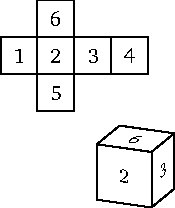
\includegraphics{taskbook-17}
	\end{figure}
\end{problem}

\begin{problem}{34.}
	Auf wie viele verschiedene Arten können $n$ Objekte angeordnet werden? 
	Für drei Objekte ($n=3$) zum Beispiel gibt es sechs verschiedene Anordnungen: $(1,2,3)$, $(1,3,2)$, $(2,1,3)$, $(2,3,1)$, $(3,1,2)$, $(3,2,1)$. 
	Wie viele Anordnungen gibt es für $n=4$? $n=5$? $n=6$? $n=10$?
	\begin{figure}[H]
	\centering
	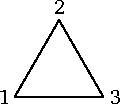
\includegraphics{taskbook-18}
	\end{figure}
\end{problem}

\begin{problem}{35.}
	Ein Würfel hat 4 Raumdiagonalen. Wie viele Permutationen dieser Diagonalen erhalten wir durch Rotation des Würfels?
	\begin{figure}[H]
	\centering
	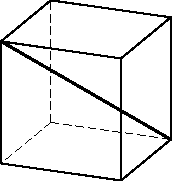
\includegraphics{taskbook-19}
	\end{figure}
\end{problem}

\begin{problem}{36.}
	Ist die Differenz zwischen der Summe des Kubiks dreier Zahlen und des Kubiks der Summe dieser drei Zahlen immer durch 3 teilbar? 
\end{problem}

\begin{problem}{37.}
	Löse Frage 36, aber für die fünfte Potenz und Teilbarkeit durch 5, und für die siebte Potenz und Teilbarkeit durch 7. 
\end{problem}

\begin{problem}{38.}
	Berechne diese Summe:
	\begin{equation*}
	\frac{1}{1\cdot 2} + \frac{1}{2\cdot 3} + \frac{1}{3\cdot 4} + \dotsb + \frac{1}{99\cdot 100}
	\end{equation*}
	(hierbei sollte der Fehler nicht größer sein als $1\%$ der Antwort).
\end{problem}

\begin{problem}{39.}
	Beweise folgende Aussage: Zwei verschiedene Vielecke mit demselben Flächeninhalt können in eine begrenzte Anzahl von kleineren Vielecken geteilt werden, sodass aus diesen Teilen beide Vielecke geformt werden können. Beweise dieses! [Dieser Satz stimmt nicht für dreidimensionale Körper: Ein Würfel und ein Tetraeder mit gleichem Volumen können nicht in dieser Weise unterteilt werden!]
	\begin{figure}[H]
	\centering
	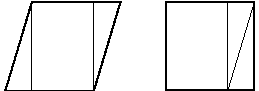
\includegraphics{q39_horizontal}\\[6pt]
	\end{figure}
\end{problem}

\begin{problem}{40.}
	Ein Parallelogramm wird auf kariertem Papier so gezeichnet, dass seine Ecken auf Ecken der Karos liegen und so, dass weder auf den Kanten noch innerhalb der Figur weitere Karo-Ecken liegen. Beweise, dass der Flächeninhalt dieses Parallelogramms genauso groß ist wie der Flächeninhalt eines der Karos. 
	\begin{figure}[H]
	\centering
	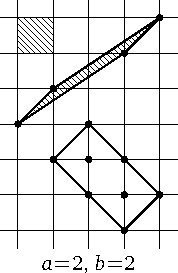
\includegraphics{taskbook-24}
	\end{figure}
\end{problem}

\begin{problem}{41.}
	Nimm dieselben Voraussetzungen an wie in Frage 40, nur dass diesmal $a$ Ecken innerhalb des Parallelogramms liegen und $b$ Ecken auf den Kanten. Berechne die Fläche dieses Parallelogramms.
\end{problem}

\begin{problem}{42.}
	Gilt die entsprechende Fassung der Aussage in Frage 40 auch für ein dreidimensionales Parallelepiped?
\end{problem}

\begin{problem}{43.}
	Die Fibonacci-Zahlen formen die Folge $1$, $1$, $2$, $3$, $5$, $8$, $13$, $21$,
	$34,\dotsc$, wobei $a_{n+2}=a_{n+1}+a_n$ für alle
	$n=1$, $2,\dotsc$ gilt ($a_n$ ist die $n$-te Zahl in der Folge). Finde den größten gemeinsamen Teiler der Zahlen $a_{100}$ und $a_{99}$.
\end{problem}

\begin{problem}{44.}
	Finde die Anzahl (Catalan-Zahl) der verschiedenen Dreieckszerlegungen eines konvexen n-Ecks durch seine sich nicht schneidenden Diagonalen.
	Zum Beispiel $c(4)=2$, $c(5)=5$, $c(6)=14$. Wie kann man $c(10)$ bestimmen?
	\begin{figure}[H]
	\centering
	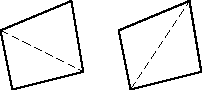
\includegraphics[scale=1]{taskbook-281}
	\qquad
	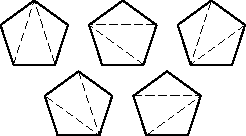
\includegraphics[scale=1]{taskbook-282}
	\end{figure}
\end{problem}

\begin{problem}{45.}
	An einem Turnier nehmen $n$ Mannschaften teil. Wenn eine Mannschaft verliert, scheidet sie aus dem Turnier aus. Der Sieger steht also nach $n-1$ Partien fest. 
	Der Ablaufplan kann symbolisch folgendermaßen notiert werden: $((a,(b,c)),d)$ würde bedeuten, dass Mannschaft $b$ zuerst  auf Mannschaft $c$ trifft, der Sieger dann gegen $a$ spielt, und der Sieger dieser Partie schließlich gegen $d$. 
	Wie viele verschiedene Ablaufpläne gibt es für 10 Mannschaften?
	\begin{itemize}
	\item Für 2 Mannschaften gibt es nur eine Möglichkeit, nämlich $(a,b)$. Die Anzahl ist 1.
	\item Bei 3 Mannschaften gibt es die Möglichkeiten $((a,b),c)$, $((a,c),b)$ oder $((b,c),a)$. Die Anzahl ist also 3.
	\item Für 4 Mannschaften gibt es die folgenden Ablaufpläne:
	\begin{equation*}
	\begin{array}{@{}cccc@{}}
		(((a,b),c),d) & \quad\;(((a,c),b),d) & \quad\;(((a,d),b),c) & \quad\;(((b,c),a),d) \\
		(((b,d),a),c) & \quad\;(((c,d),a),b) & \quad\;(((a,b),d),c) & \quad\;(((a,c),d),b) \\ 
		(((a,d),c),b) & \quad\;(((b,c),d),a) & \quad\;(((b,d),c),a) & \quad\;(((c,d),b),a) \\
		((a,b),(c,d)) & \quad\;((a,c),(b,d)) & \quad\;((a,d),(b,c))
	\end{array}
	\end{equation*}
	\end{itemize}
\end{problem}

\begin{problem}{46.}
	Verbinde die Punkte $1, 2, \dotsc, n$ mit $n-1$ Linien. Wie viele verschiedene Bäume können so entstehen? (Der Fall $n=5$ ist schon sehr interessant!)

	$n=2$:\quad 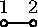
\includegraphics{taskbook-291}\,,\quad die Anzahl ist 1; 

	$n=3$:\quad 
	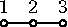
\includegraphics{taskbook-292}\,,\quad 
	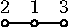
\includegraphics{taskbook-293}\,,\quad 
	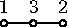
\includegraphics{taskbook-294}\,,\quad 
	die Anzahl ist 3;

	$n=4$:\quad
	$\vcenter{\hbox{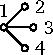
\includegraphics{taskbook-295}}}$,\quad
	$\vcenter{\hbox{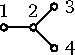
\includegraphics{taskbook-296}}}$,\quad
	$\vcenter{\hbox{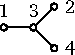
\includegraphics{taskbook-297}}}$,\quad
	$\vcenter{\hbox{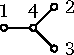
\includegraphics{taskbook-298}}}$,\quad
	$\vcenter{\hbox{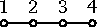
\includegraphics{taskbook-299}}\hbox{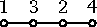
\includegraphics{taskbook-290}}
	\vskip-8pt
	\hbox to50bp{\dotfill}}$,\\ 
	\null\hspace{\parindent}\phantom{$n=4$:}\quad die Anzahl ist 16.
\end{problem}

\begin{problem}{47.}
	Eine Permutation $(x_1,x_2, \dots,x_n)$ der Zahlen $\{1, 2, \dotsc, n\}$ wird eine
	\emph{Schlange} mit Länge $n$ genannt, wenn $x_1<x_2>x_3<x_4 \dotsb$.

	{\noindent\sc beispiel:\nopagebreak}
	\begin{equation*}
	\begin{aligned}[t]
	&\begin{aligned}[t] n=2, \text{\ \ nur\ \ } 1<2, \end{aligned} &&\text{die Anzahl der Schlangen ist }1, \\
	&\hskip-\nulldelimiterspace\mathord{\left.\begin{aligned} n=3, \hphantom{\text{\ \ nur\ \ }} 1&<3>2 \\ 
	2&<3>1\end{aligned} \right\}}, && \text{die Anzahl der Schlangen ist }2, \\[2pt]
	&\hskip-\nulldelimiterspace\mathord{\left.\begin{aligned} n=4, \hphantom{\text{\ \ nur\ \ }} 1&<3>2<4 \\ 
	1&<4>2<3 \\ 
	2&<3>1<4 \\ 
	2&<4>1<3 \\ 
	3&<4>1<2\end{aligned} \right\}},
	&&\text{die Anzahl der Schlangen ist }5. \\
	\end{aligned}
	\end{equation*}
	Wie viele Schlangen der Länge 10 gibt es?
\end{problem}

\begin{problem}{48.}
	Sei $s_n$ die Anzahl der Schlangen mit Länge $n$, also zum Beispiel: 
	\begin{equation*}
	s_1=1, \quad s_2=1, \quad s_3=2, \quad s_4=5, \quad s_5=16, \quad s_6=61.
	\end{equation*}
	Beweise, dass die Taylorreihe des Tangens wie folgt aussieht: 
	\begin{equation*}
	\tan x=1\, \frac{x^1}{1!}+2\, \frac{x^3}{3!}+16\, \frac{x^5}{5!}+\dots=
	\textstyle\sum\limits_{k=1}^{\infty} s_{2k-1}\, \frac{x^{2k-1}}{(2k-1)!}.
\end{equation*}
\end{problem}

\begin{problem}{49.}
	Finde die Summe dieser Reihe:
	\begin{equation*}
	1+1\, \frac{x^2}{2!}+5\, \frac{x^4}{4!}+61\, \frac{x^6}{6!}+\dots=
	\textstyle\sum\limits_{k=0}^{\infty} s_{2k}\,\frac{x^{2k}}{(2k)!}.
\end{equation*}
\end{problem}

\begin{problem}{50.}
	Für $s>1$, beweise folgende Gleichung:
	\begin{equation*}
	\textstyle\prod\limits_{p=2}^{\infty} \frac{1}{1-\frac{1}{p^s}}=\textstyle\sum\limits_{n=1}^{\infty} \frac{1}{n^s}
	\end{equation*}
	(Das Produkt auf der linken Seite läuft über alle Primzahlen $p$, die Summe rechts wird über alle natürlichen Zahlen~$n$ gebildet.)
\end{problem}

\begin{problem}{51.}
	Finde die Summe dieser Reihe:
	\begin{equation*}
	1+ \frac{1}{4}+ \frac{1}{9}+\dots=\textstyle\sum\limits_{n=1}^{\infty} \frac{1}{n^2}.
	\end{equation*}
	[Beweise, dass die Antwort $\nicefrac{\pi^2}{6}$, ist, also schätzungsweise $\nicefrac{3}{2}$].
\end{problem}

\begin{problem}{52.}
	Sei $R$ der Radius einer Kreisscheibe und $p$ und $q$ zwei ganze Zahlen, die der Ungleichung $p^2+q^2 \leqslant R^2$ genügen. Wie groß ist die Wahrscheinlichkeit, dass der Bruch $\nicefrac{p}{q}$ in gekürzter Form vorliegt?
	
	Dazu zählen wir die Punkte mit ganzzahligen Koordinaten innerhalb der Kreis\-schei\-be, deren größter gemeinsamer Teiler 1 ist. Wir nennen diese Anzahl $N(R)$ . (Die Anzahl $N$ der Punkte hängt vom Radius $R$ ab, das machen wir durch die Schreibweise $N(R)$ deutlich.)  Weiterhin sei $M(R)$ die Gesamtanzahl der Punkte mit ganzzahligen Koordinaten innerhalb der Kreisscheibe $(M(R) \sim \pi R^2)$. Die Wahrscheinlichkeit, dass der Bruch $\nicefrac{p}{q}$ nicht mehr gekürzt werden kann, ist dann der Grenzwert des Bruches $\nicefrac{N(R)}{M(R)}$.
	\begin{figure}[H]
	\footnotesize
	\centering
	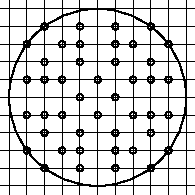
\includegraphics{taskbook-36}\\
	$M(5)=81$, $N(5)=44$, $\nicefrac{N}{M} = \nicefrac{44}{81}$
	\end{figure}
\end{problem}

\begin{problem}{53.}
	Finde den Grenzwert des Quotienten $\nicefrac{a_{n+1}}{a_n}$ für die Fibonacci Zahlen $a_n$ von Aufgabe 43, wenn $n$ gegen unendlich geht:
	\begin{equation*}
	\frac{a_{n+1}}{a_n}=2,\ \frac 32,\ \frac53, \ \frac85, \ \frac{13}8,
	\ \frac{34}{21}.
	\end{equation*}
	[Die Antwort ist der \enquote{Goldene Schnitt},
	$\frac{\sqrt{5}+1}{2} \approx 1{,}618$. (Dies ist das Tei\-lungs\-ver\-hält\-nis der zwei Längen eines Rechtecks $ABCD$, das selbstähnlich zu demjenigen Rest ist, den man erhält, wenn man das Quadrat $ABPQ$ davon abschneidet: 
	$\frac{AB}{BC}=\frac{PC}{CD}$.) Was hat der Goldene Schnitt mit einem regelmäßigen Fünfeck und einem Pentagramm (fünfzackiger Stern) zu tun?]
	\begin{figure}[H]
	\centering
	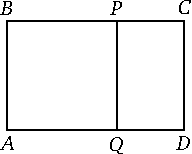
\includegraphics{taskbook-37}
	\end{figure}
\end{problem}

\begin{problem}{54.}
	Bestimme den Grenzwert des unendlichen Kettenbruches
	\begin{equation*}
	1+\cfrac{1}{2+\cfrac{1}{1+\cfrac{1}{2+\cfrac{1}{1+\cfrac{1}{2+\ldots}}}}}=
	a_0+\cfrac{1}{a_1+\cfrac{1}{a_2+\cfrac{1}{a_3+\dots}}}
	%\quad
	%\smash{
	%%\medmath
	%{\left[\begin{aligned} &a_{2k}=1 \\[-\jot] &a_{2k+1}
	%=2 \end{aligned}\right]} }
	\end{equation*}
	mit $a_{2k}=1$ und $a_{2k+1}=2$. In anderen Worten, bestimme den Grenzwert des Bruches
	\begin{equation*}
	a_0+\cfrac{1}{a_1+\cfrac{1}{a_2+{\atop{\ddots \atop {}} + \cfrac{1}{a_n}}}}
	\end{equation*}
	für $n \to \infty$).
\end{problem}

\begin{problem}{55.}
	Bestimme die Polynome 
	\begin{equation*}
	y=\cos 3 (\arccos x),\ y=\cos 4 (\arccos x),\ 
	y=\cos n (\arccos x),
	\end{equation*}
	wobei $|x| \leqslant 1$.
\end{problem}

\begin{problem}{56.}
	Bestimme die Summe der $k$-ten Potenz der $n$-ten Einheitswurzeln.
\end{problem}

\begin{problem}{57.}
	Zeichne die Kurven der folgenden Gleichungen in Parameterdarstellung in ein Koordinatensystem: 
	\begin{equation*}
	\{x=\cos 2t, y=\sin 3t\},\quad 
	\{x=t^3-3t, y=t^4-2t^2\}.
	\end{equation*}
	(Dafür kannst du z.\,B.\ eine Wertetabelle erstellen. Setze verschiedene Werte für $t$ ein und beobachte, wie sich die Punkte im Koordinatensystem verhalten. Erkennst du Regelmäßigkeiten?)
\end{problem}

\begin{problem}{58.}
	Bestimme den Wert des Integrals $\int_0^{2\pi} \sin^{100} x\,dx$, wobei der Fehler nicht größer sein sollte als $10\%$ der Antwort.
\end{problem}

\begin{problem}{59.}
	Bestimme den Wert des Integrals $\int_1^{10} x^x\,dx$, wobei der Fehler nicht größer sein sollte als $10\%$ der Antwort.
\end{problem}

\begin{problem}{60.}
	Bestimme den Flächeninhalt $S$ eines Dreiecks mit den Winkeln $(\alpha, \beta, \gamma)$ auf einer Kugel mit Radius 1, wobei die Seiten des Dreiecks auf Großkreisen liegen (Schnitte der Kugel mit Ebenen, die den Mittelpunkt der Kugel enthalten).

	\noindent\textsc{antwort:} $S=\alpha+\beta+\gamma-\pi$ (z.\,B.\ für ein Dreieck mit drei rechten Winkeln ist $S=\nicefrac{\pi}{2}$. In diesem Fall beträgt die Fläche des Dreiecks ein Achtel der Gesamtoberfläche der Kugel).
	\begin{figure}[H]
	\null\hfill
	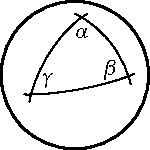
\includegraphics{taskbook-44}
	\hfill
	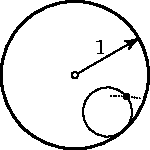
\includegraphics{taskbook-45}
	\hfill\null
	\end{figure}
\end{problem}

\begin{problem}{61.}
	Ein Kreis mit Radius $r$ rollt (ohne zu rutschen) innerhalb eines Kreises mit Radius 1 ab.
	Zeichne die vollständige Bahn eines Punktes auf dem rollenden Kreis für $r=\nicefrac{1}{3}$, für $r=\nicefrac{1}{4}$, für $r=\nicefrac{1}{n}$ und für $r=\nicefrac{1}{2}$. (Solche Bahnen nennen sich Hypozykloide.)
	
	{\noindent\sc tipp:} Führe dieses Gedankenexperiment zunächst mit einem rollenden Kreis auf einer Geraden durch. Die entstehende Kurve heißt Zykloide. Übertrage diesen Fall nun auf das ursprüngliche Problem.
\end{problem}

\begin{problem}{62.}
	Wie groß ist die Wahrscheinlichkeit, dass in einer Klasse mit $n$ Schülern zwei Schüler am gleichen Tag Geburtstag haben? Findest du sie hoch oder niedrig? 
	Bei welcher Schülerzahl liegt die Wahrscheinlichkeit in etwa bei $\nicefrac{1}{2}$?
\end{problem}

\begin{problem}{63.}
	Das Snelliussche Brechungsgesetz besagt, dass der Winkel $\alpha$ zwischen einem Lichtstrahl und der Senkrechten zu der Oberfläche eines mehrschichtigen Mediums durch die folgende Gleichung bestimmt wird: 
	\begin{equation*}
		n(y) \sin \alpha=\text{const}.
	\end{equation*}
	Hierbei ist $n(y)$ der Brechungsindex einer Schicht auf der Höhe $y$. (Der Index $n$ ist umgekehrt proportional zu der Lichtgeschwindigkeit im Medium, wenn die Geschwindigkeit im Vakuum als 1 angenommen wird; in  Wasser z.\,B.\ ist $n$ unabhängig von der Höhe $y$ und nimmt den Wert $n=\nicefrac{4}{3}$ an.)
	\begin{figure}[H]
	\null\hfill
	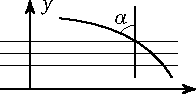
\includegraphics{taskbook-47}
	\hfill
	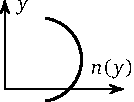
\includegraphics{taskbook-471}
	\hfill\null
	\end{figure}

	Zeichne die Bahnen der Lichtstrahlen im Medium “Luft über einer Wüste”, wobei der Index $n(y)$ bei einer bestimmten Höhe sein Maximum erreicht. (Die Lösung zu dieser Frage erklärt die Erscheinung einer Fata Morgana in der Wüste).
\end{problem}

\begin{problem}{64.}
	Wir betrachten ein spitzwinkliges Dreieck $ABC$. Finde das Dreieck $KLM$ mit dem kleinstmöglichen Umfang, das so in $ABC$ eingeschrieben ist, dass Ecke $K$ auf der Strecke $AB$, Ecke $L$ auf $BC$ und Ecke $M$ auf $CA$ liegt. 
	\begin{figure}[H]
	\centering
	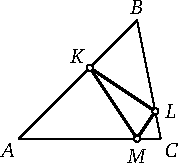
\includegraphics{taskbook-48} 
	\end{figure}

	\noindent\textsc{bemerkung:} Für nicht-spitzwinklige Dreiecke ist die Antwort nicht so elegant wie für spitzwinklige.
\end{problem}

\begin{problem}{65.}
	Berechne den Mittelwert der Funktion $\nicefrac{1}{r}$ (wobei $r^2\,=x^2\,+y^2+z^2$, $r$ ist der Abstand zum Ursprung)  auf der Kugel mit Radius $R$ und Mittelpunkt $(X,Y,Z)$.

	\noindent\textsc{hinweis:} Dieses Problem ist dem Newtonschen Gravitationsgesetz und dem Coulombschen Gesetz für Elektrizitätstheorie verwandt. In der zweidimensionalen Version dieses Problems ist die Funktion durch $\ln r$ und die Kugel durch einen Kreis zu ersetzen.
\end{problem}

\begin{problem}{66.}
	Aus der Tatsache, dass $2^{10}=1024 \approx 10^3$ ist, kann man schlussfolgern, dass $\log_{10} 2 \approx 0.3$. Schätze den Unterschied zwischen $\log_{10} 2$ und $0.3$ und berechne $\log_{10} 2$ auf drei Dezimalstellen genau. 
\end{problem}

\begin{problem}{67.}
	Bestimme $\log_{10} 4$, $\log_{10} 8$, $\log_{10} 5$, $\log_{10} 50$, $\log_{10} 32$, $\log_{10} 128$, $\log_{10} 125$, $\log_{10} 64$ mit der gleichen Genauigkeit.
\end{problem}

\begin{problem}{68.}
	Wenn wir $7^2$ durch $50$ annähern, schätze den Wert von $\log_{10} 7$.
\end{problem}

\begin{problem}{69.}
	Bestimme $\log_{10} 9$, $\log_{10} 3$, $\log_{10} 27$, $\log_{10} 6$, $\log_{10} 12$, wobei $\log_{10} 64$ und $\log_{10} 7$ gegeben sind.
\end{problem}

\begin{problem}{70.}
	Es ist $\ln (1+x) \approx x$, wobei $\ln$ für $\log_e$ steht\footnote{Die Eulerzahl $e = 2{,}71828\dots$ ist definiert als der Grenzwert der Folge $\left(1+\frac1n\right)^n$ für $n\to \infty$, und ist gleich der Summe der Reihe 
	$1+\frac 1{1!} +\frac 1{2!}+\frac 1{3!}+\dots{}$ Sie kann auch anhand der Formel für $\ln (1+x)$: $\lim\limits_{x\to 0}\frac{\ln(1+x)}{x} = 1$ definiert werden.}. Bestimme den Wert für $\log_{10} e$ und $\ln 10$ mit Hilfe der Gleichung 
	%
	\begin{equation*}
	\log_{10} a=\frac{\ln a}{\ln 10}
	\end{equation*} 
	und der Werte für $\log_{10} a$, die vorher berechnet wurden (zum Beispiel für $a=\nicefrac{128}{125}$, $\nicefrac{1024}{1000}$ und so weiter).
	
	[Die Antworten zu den Aufgaben 65--69 liefern eine Tabelle für 4-stellige Logarithmen von einer beliebigen Zahl, mit Hilfe der Produkte von Zahlen, die im Voraus als Grunddaten bestimmt wurden, sowie der Formel 
	\begin{equation*}
	\ln (1+x) \approx x-\frac{x^2}{2}+\frac{x^3}{3}-\frac{x^4}{4}+\dots,
	\end{equation*}
	um Fehler zu korrigieren.] (Auf diese Weise stellte Newton eine Tabelle von 40-stelligen Logarithmen zusammen!)
\end{problem}

\begin{problem}{71.}
	Betrachte die Folge der Zweierpotenzen: $1$, $2$, $4$, $8$, $16$, $32$, $64$, $128$, $256$, $512$, $1024$, $2048, \dots$ Unter den ersten zwölf Zahlen sind vier, die mit 1 anfangen, aber keine, die mit 7 beginnt. 

	Beweise, dass für den Grenzwert $n \to \infty$ die erste Ziffer der Zahlen $2^m$,
	$0\leqslant m \leqslant n$ mit einer bestimmten Frequenz auftreten: 
	$p_1 \approx 30\%$, $p_2 \approx 18\%$, $\dots$, $p_9 \approx 4\%$.
\end{problem}

\begin{problem}{72.}
	Betrachte die erste Ziffer der Dreierpotenzen: $1$,
	$3$, $9$, $2$, $8$, $2$, $7, \dots$ . Beweise, dass für den gleichen Grenzwert wie in Aufgabe 71 ebenfalls bestimmte Frequenzen auftreten, und zwar die gleichen wie für die Zweierpotenzen. Finde die genauen Werte für $p_1, \dots, p_9$.

	\noindent\textsc{hinweis:} Die erste Ziffer einer Zahl $x$ ist durch den Dezimalteil der Zahl 
	$\log_{10} x$ bestimmt. Es genügt also, den Dezimalteil der Zahlen $m \alpha$ zu betrachten, wobei $\alpha=\log_{10} 2$ ist.

	Beweise, dass diese Dezimalteile gleichmäßig über das Intervall von $0$ bis $1$ verteilt sind: Für ein Teilintervall $A$ des Intervalls von $0$ bis $1$ sei $k_n(A)$ die Anzahl der Dezimalteile der Zahlen $m\alpha$, $0 \leqslant m < n$, die in $A$ liegen. Zeige, dass $\lim(k_n(A)/n)=(\text{Länge des Teilintervalls $A$})$ für $n\rightarrow \infty$ gilt.
\end{problem}

\begin{problem}{73.}
	Sei $M$ beschränkt und $g\colon M \to M$ eine glatte, injektive Abbildung, die Flächen erhält (bzw. im mehrdimensionalen Fall analog dazu das Volumen). 

	%My contribution: (???) Sei $g\colon M \to M$ eine glatte, injektive Abbildung von dem beschränktes Gebiet $M$ auf sich selbst die ....
	 
	Betrachte einen beliebigen Punkt in $M$ und eine beliebige Umgebung $U$ um diesen Punkt. Zusätzlich sei $N$ eine beliebige natürliche Zahl. 
	Zeige, dass es dann einen weiteren Punkt $x$ in $U$ gibt, sodass für ein $T\geq N$ gilt, dass $g^T (x)$, d.\,h.\ wir betrachten $g(g(\dots (x))$, wobei $g$ insgesamt $T$ mal angewendet wird, wieder in $U$ liegt (\enquote{Poincaréscher Wiederkehrsatz}).
	%Zeige, dass für jeden Punkt in $M$ und jede Umgebung $U$ von $p$ für eine beliebige natürliche Zahl $N$ ein weiterer Punkt $x$ in $M$ existiert, 

	%Beweise, dass in der Umgebung $U$ von jedem beliebigen Punkt von $M$ und für beliebige $N$ ein Punkt $x$ existiert, so dass $g^T x$ auch in $U$ liegt für bestimmte ganze Zahlen $T>N$ (\enquote{Das Rekurrenz-Theorem}).

	%??? My Version:
	%Beweise dass zu jedem Punkt in $M$, zu jeder Umgebungen $U$ dieses Punktes und für alle $N$ es ganze Zahlen $T>N$ gibt, für die gilt dass $g^T x$ sich auch in $U$ gefindet. (\enquote{poincarésche Wiederkehrsatz}).
\end{problem}

\begin{problem}{74.}
	Sei $M$ die Oberfläche eines Torus (ein Torus sieht aus wie ein Donut). Man kann ihn sehr einfach formal beschreiben, indem man als Koordinatenachsen diese zwei Kreise wählt. 
	\begin{figure}[H]
	\centering
	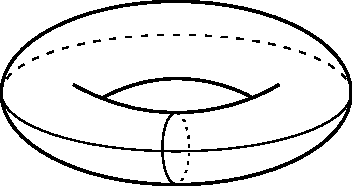
\includegraphics{74_torus} 
	\end{figure}

	Punkte mit Koordinaten $(a,0)$ beispielsweise liegen dann auf dem horizontalen Kreis, Punkte mit Koordinaten $(0,b)$ auf dem vertikalen. 
	Da wir nach einer vollen Umdrehung ($360^\circ$ oder $2\pi$) entlang einer der Kreise wieder am Ausgangspunkt ankommen, genügt es, die Koordinaten modulo $2\pi$ zu betrachten.
	
	Sei also der Torus durch die Koordinaten ($\alpha$ mod $2\pi$, $\beta$ mod $2\pi$) beschrieben und $g: M\to M$ so, dass
	\begin{equation*}
		g(\alpha, \beta)=(\alpha+1, \beta+ \sqrt{2}).
	\end{equation*}
	Zeige, dass die Folge $\{g^T (x)\}$ für alle $x$ in $M$ überall im Torus dicht liegt, wobei $T$ die Werte $1,2,\dots$ annehmen soll. 

	%Sei $M$ die Torusoberfläche (mit Koordinaten $\alpha$ (mod $2\pi$), $\beta$ (mod $2\pi$)) und $g(\alpha, \beta)=(\alpha+1, \beta+ \sqrt{2})$ (mod $2\pi$). Beweise dass die Folge von Punkten $\{g^T (x)\}$, $T=1, 2, \dots$ überall in dem Torus dicht liegt.
\end{problem}

\begin{problem}{75.}
Mit den gleichen Voraussetzungen wie in Aufgabe 74 sei nun $f: M\to M$ so, dass
%Sei nun, in Bezug auf Aufgabe 74, 
\begin{equation*}
f(\alpha, \beta)=(2\alpha+\beta,\alpha+\beta) \pmod {2\pi}.
\end{equation*}
Zeige, dass eine Teilmenge des Torus existiert, die überall dicht ist und aus periodischen Punkten bezüglich $f$ besteht. 
%Beweise die Existenz einer überall dichten Untermenge, die aus periodischen Punkten $x$ des Torus' besteht
(\enquote{Periodisch} heißt, dass $f^{T (x)} (x)=x$ gilt für gewisse natürliche Zahlen $T(x)$. Die Zahl $T$ hängt hierbei von dem Punkt $x$ ab; diese Abhängigkeit wird durch die Schreibweise $T(x)$ ausgedrückt.)


\end{problem}

\begin{problem}{76.}
Wir nehmen die gleichen Voraussetzungen wie in Aufgabe 74 an und betrachten die Abbildung $f$ aus Aufgabe 75. Beweise, dass für fast alle Punkte $x$ auf dem Torus die Folge der Punkte $\{f^T (x)\}$, $T=1, 2, \dots$ überall auf dem Torus dicht ist. 
%(Punkte $x$ ohne diese Eigenschaft bilden eine Menge mit Maß Null). 


\end{problem}

\begin{problem}{77.}
Wir verwenden die Notation aus den Aufgaben 74 und 76. Beweise, dass die Folge $\{g^T (x)\}$, $T=1, 2, \dots$ über den Torus gleichförmig (uniform) verteilt ist. Damit ist folgendes gemeint: 
Wir betrachten eine Teilmenge $A$ von $M$ und zählen die Punkte der Folge bis zum $n$-ten Folgenglied, die in $A$ liegen. Diese Anzahl nennen wir $k_n(A)$. 
Damit die Folge gleichmäßig verteilt ist, muss nun 
\[
\lim_{n \to \infty} \frac{k_n(A)}{n}=\frac{{\text{Fläche}} (A)}{{\text{Fläche}} (M)}
\]
%\[
%\lim_{n \to \infty} \frac{k_n(A)}{n}=\frac{\operatorname{mes} A}{\operatorname{mes} M}
%\]
gelten. 
%(zum Beispiel für einen Jordan-messbaren Definitionsbereich $A$ mit Maß $\operatorname{mes} A$).
\end{problem}
\ 

\ 

\ 

\noindent\textsc{anmerkung zu aufgabe }\oldstylenums{13}. Ich habe in meinem Beitrag zur Weihnachts"=Jubiläumsausgabe im Jahr 2000 der Zeitschrift \enquote{Physics"=Uspekhi} versucht, anhand dieser Aufgabe die unterschiedlichen Herangehensweisen darzustellen, die man typischerweise bei Mathematikern und Physikern findet. Der Erfolg übertraf meine Erwartungen. Die Redaktion war nicht in der Lage, das Problem zu lösen und änderte die Aufgabenstellung so, wie sie ihrer Meinung nach richtig war, um die Lösung \SI{4}{\mm} zu erhalten: Statt \enquote{von der ersten Seite im Band 1 bis zur letzten Seite im Band 2} hieß es in der Veröffentlichung \enquote{von der \emph{letzen} Seite im Band 1 bis zur \emph{ersten} Seite im Band 2}. 

Diese wahre Geschichte ist so unglaublich, dass ich sie hier erwähne: der Beweis ist die Erstveröffentlichung von der Redaktion.

\clearpage
\null\vfill
%\null\hfill\parbox{\textwidth}%
{%
\noindent
Übersetzung Russisch - Englisch:\\
\null\quad Victor Goryunov und Sabir Gusein-Zade\\
\\
Übersetzung Englisch - Deutsch:\\
\null\quad David Grünberg, Lilian Hueber und Lea Renner\\
\\
Ergänzungen und Glossar:\\
\null\quad Lea Renner\\
\\
Design und Layout:\\
\null\quad Konrad Renner und Christian Stussak\\
\\
\\
Aus dem russischen Original:\\
\null\quad В. И. Арнольд: Задачи для детей от 5 до 15 лет\\
\null\quad Moskau, MCCME, 2004\\
\null\quad ISBN 5-94057-183-2\\
\\
\\
Bildquelle:\\ 
\null\quad Archiv des Mathematischen Forschungsinstituts Oberwolfach\\
\\
\\
Dieses Buch ist unter der Lizenz CC BY-NC-SA 3.0 auf der IMAG\-I\-NARY-Plattform erhältlich: \href{http://www.imaginary.org/background-materials}{www.imaginary.org/background-materials}.
}
\clearpage

\section*{Glossar}
\begin{description}
\item[dicht] Eine Teilmenge $A$ von einer \enquote{großen} Menge $M$ liegt dicht in $M$, wenn man jedes Element aus $M$ mit Elementen aus $A$ beliebig gut approximieren kann (sprich: Wenn man mit Elementen aus $A$ beliebig dicht an jedes Element aus $M$ herankommt). 

Zum Beispiel liegt die Menge der rationalen Zahlen $\mathbb{Q}$ dicht in der Menge der reellen Zahlen $\mathbb{R}$, d.\,h.\ jede reelle Zahl kann beliebig gut durch einen Bruch angenähert werden. 

\item[Einheitswurzel] Eine $n$-te Einheitswurzel ist eine Zahl, die zur $n$-ten Potenz 1 ergibt (in Formeln: eine Zahl $z$, sodass $z^n = 1$). 

Zum Beispiel ist 1 eine n-te Einheitswurzel für jede natürliche Zahl $n$, denn es gilt $1^n = 1$. 
Wenn $n$ gerade ist, so ist zusätzlich $-1$ eine $n$-te Einheitswurzel, denn dann ist $(-1)^n = 1$. 

Im Allgemeinen findet man Einheitswurzeln im Bereich der komplexen Zahlen. Dieses ist der nächstgrößere Zahlbereich über der Menge der reellen Zahlen $\mathbb{R}$. 
Es kann spannend sein, sich dort etwas einzulesen.

\item[Folge] Eine Folge ist eine Auflistung von nummerierten Objekten, die einer Bildungsvorschrift unterliegt. Die Folge selbst wird als $(a_n) = a_1,a_2,a_3,\dots $ geschrieben, das Zeichen $a_n$ bezeichnet das $n$-te Folgenglied. 

Beispiele: 
\begin{itemize}
\item Die natürlichen Zahlen mit der Bildungsvorschrift $a_n = n$:
\begin{equation*}
1,2,3,4,5,\dots{}
\end{equation*}
Man kann auch einzelne Folgeglieder herausgreifen, z.\,B.\ $a_{14} = 14$. 
\item Die Fibonacci-Zahlen mit der Bildungsvorschrift $a_n = a_{n-1}+a_{n-2}$ und dem Start $a_1 = a_2 = 1$:
\begin{equation*}
1,1,2,3,5,8,13,\dots{}
\end{equation*}
\item Die Folge, die durch die Bildungsvorschrift $a_n = f^n(x)$ für die Funktion $f(x) = 2x-1$ gegeben ist. Hierfür brauchen wir natürlich einen Startwert für das $x$, z.\,B.\ $x=2$: 
\begin{equation*}
a_1 = f(2) = 3,\ a_2 = f(3) = 5,\ a_3 = f(5) = 9,\dots
\end{equation*}
Anders geschrieben lautet die Folge also $3,5,9,17,33\dots{}$
\end{itemize}

\item[glatte Abbildung] Laut der mathematischen Definition heißt eine Abbildung glatt, wenn sie unendlich oft differenzierbar ist. 
Zum \nopagebreak Beispiel ist jedes Polynom glatt: 
\[f(x) = x^2 + 3,\ f'(x) = 2x,\ f''(x) = 2, \]
\[f'''(x) = f^{(n)}(x) = 0 \text{ für alle natürlichen Zahlen } n.\]
Auch die $e$-Funktion gehört zu den glatten Abbildungen: 
\[g(x) = e^x, g'(x) = g^{(n)}(x) = e^x \text{ für alle natürlichen Zahlen } n.\]
Ein Beispiel für eine Funktion, die nicht glatt ist, ist die Betragsfunktion $h(x) = |x|.$ Sie hat bei $x=0$ eine \enquote{Spitze} und kann dort nicht differenziert werden. 

Anschaulich kann das Wort \enquote{glatt} bei Funktionen wörtlich verstanden werden: Der Graph einer glatten Funktion hat keine Spitzen und lässt sich in einem Strich zeichnen. 

\item[injektiv] Eine Abbildung, die kein Element aus dem Zielbereich öfter als einmal trifft, heißt injektiv. 
Zum Beispiel ist jede Permutation injektiv (siehe Permutation). 

Beispiele: 
\begin{figure}[H] 
\centering 
\def\svgwidth{200pt} 
\input{glossar_injektiv.pdf_tex} 
\end{figure}
Die Funktion $f(x) = x^2$ ist nicht injektiv, wenn man als Definitionsbereich die ganze reelle Achse zulässt. Dann ist nämlich $f(-1) = f(1) = 1$, die 1 wird also zweimal getroffen. 

\item[konvex] Mathematikerinnen und Mathematiker nennen eine Figur (z.\,B.\ ein Polyeder) konvex, wenn man zwischen zwei beliebigen Punkten der Figur eine gerade Linie zeichnen kann und die gesamte Linie im Inneren der Figur liegt. 
Anschaulich gesprochen ist eine konvexe Figur überall nach außen gewölbt. 

Beispiele: 
\begin{figure}[H] 
\centering 
\def\svgwidth{270pt} 
\input{glossar_konvex.pdf_tex} 
\end{figure} 

\item[modulo] Wir schreiben $a \operatorname{mod} b$ und meinen den Rest, der übrigbleibt, wenn $a$ durch $b$ geteilt wird. 
Ähnlich wie ein Gleichheitszeichen funktioniert in diesem Zusammenhang das Symbol \enquote{$\equiv$}. 

$c\equiv a \operatorname{mod} b$ (sprich: $c$ ist kongruent zu $a$ modulo $b$) bedeutet, dass $c$ und $a$ beim Teilen durch $b$ denselben Rest lassen. 

Beispiele: $7\equiv 1\operatorname{mod} 6,\ 11\equiv 3\operatorname{mod} 4$.

\item[Permutation] Eine Permutation ist eine Abbildung, bei der die Zahlen $1,2,\dots,n$ so auf die Zahlen $1,2,\dots,n$ abgebildet werden, dass jede Zahl in der Bildmenge getroffen wird. 

Beispiele:
\begin{figure}[H] 
\centering 
\def\svgwidth{200pt} 
\input{glossar_permutation.pdf_tex} 
\end{figure} 

\item[Produktzeichen] Ähnlich wie das Summenzeichen ist das Produktzeichen $\prod$ eine Kurzschreibweise für \enquote{diese Zahlen werden miteinander multipliziert}. Auch hier werden die Grenzen unter und über das Symbol geschrieben. 

Beispiele: 
\begin{gather*}
\prod\limits_{k=3}^5 k = 3\cdot 4\cdot 5 = 60,\\
\prod\limits_{m=4}^7 m^2 - m = (4^2-4)\cdot(5^2-5)\cdot (6^2-6) \cdot (7^2-7)= 302\,400.
\end{gather*}
\item[Summenzeichen] Das Summenzeichen $\sum$ ist eine Kurzschreibweise für die Aussage \enquote{diese Zahlen werden addiert}. 
Damit man weiß, von wo bis wo man addieren muss, werden die Grenzen unter (der Anfang) und über (das Ende) das Zeichen geschrieben:
\begin{equation*}
\sum\limits_{i=1}^5 i,
\end{equation*}
sprich \enquote{die Summe über $i$ von 1 bis 5}, heißt also, dass alle Zahlen von 1 bis 5 aufaddiert werden sollen. 

Beispiele: \[\sum\limits_{i=7}^{11} i= 7+8+9+10+11 = 45,\] 
\[\sum\limits_{i=1}^3 i\cdot (i+2) = 1\cdot (1+2) + 2\cdot (2+2) + 3\cdot (3+2) = 26.\] 
Man kann auch Summen betrachten, die keine obere Grenze haben, die also bis unendlich gehen. Man schreibt dann $\sum\limits_{i=1}^\infty$. 
\end{description}
%
\clearpage
\thispagestyle{empty}
\null
\includepdf[pages={4,1}]{"cover_de_DE"}
\end{document}
